%===============================================================
%  Korean A4 XeLaTeX Template
%  컴파일: xelatex (VS Code LaTeX Workshop 기본 컴파일러)
%===============================================================
\documentclass[12pt, a4paper]{article}

%---------------------------------------------------------------
% 한글 폰트 및 언어 설정
%---------------------------------------------------------------
\usepackage{fontspec}
\usepackage{xeCJK}

% 한글 폰트 (Windows 기본 폰트)
\setCJKmainfont{Malgun Gothic}          % 본문 한글: 맑은 고딕
\setCJKsansfont{Malgun Gothic}
\setCJKmonofont{Malgun Gothic}

% 영문 폰트
\setmainfont{Times New Roman}
\setsansfont{Arial}
\setmonofont{Courier New}

%---------------------------------------------------------------
% 페이지 레이아웃 (A4)
%---------------------------------------------------------------
\usepackage[
  a4paper,
  top=25mm, bottom=25mm,
  left=25mm, right=25mm,
  headheight=14pt
]{geometry}

%---------------------------------------------------------------
% 수식 패키지
%---------------------------------------------------------------
\usepackage{amsmath, amssymb, amsthm}
\usepackage{mathtools}

%---------------------------------------------------------------
% TikZ / 그림 패키지
%---------------------------------------------------------------
\usepackage{tikz}
\usepackage{pgfplots}
\pgfplotsset{compat=1.18}

% 자주 쓰는 TikZ 라이브러리
\usetikzlibrary{
  arrows.meta,
  calc,
  patterns,
  decorations.pathmorphing,
  decorations.markings,
  angles,
  quotes,
  shapes.geometric,
  positioning,
  intersections
}

%---------------------------------------------------------------
% 색상 / 박스 환경
%---------------------------------------------------------------
\usepackage{xcolor}
\usepackage[most]{tcolorbox}

% 색상 정의
\definecolor{myblue}{RGB}{31, 78, 121}
\definecolor{mygreen}{RGB}{0, 112, 54}
\definecolor{mygray}{RGB}{89, 89, 89}
\definecolor{myorange}{RGB}{197, 90, 17}
\definecolor{mypurple}{RGB}{112, 48, 160}
\definecolor{lightblue}{RGB}{219, 229, 241}
\definecolor{lightgreen}{RGB}{226, 240, 217}
\definecolor{lightgray}{RGB}{242, 242, 242}
\definecolor{lightorange}{RGB}{255, 235, 211}
\definecolor{lightpurple}{RGB}{240, 230, 255}

%----------- tcolorbox 환경 정의 ----------------------------

% 유도 / 설명 박스 (회색)
\newtcolorbox{derivbox}[1][]{
  colback=lightgray, colframe=mygray,
  fonttitle=\bfseries\small,
  title={#1},
  left=4pt, right=4pt, top=4pt, bottom=4pt,
  boxrule=0.6pt
}

% 예제 / 풀이 박스 (초록)
\newtcolorbox{samplebox}[1][]{
  colback=lightgreen, colframe=mygreen,
  fonttitle=\bfseries\small,
  title={#1},
  left=4pt, right=4pt, top=4pt, bottom=4pt,
  boxrule=0.6pt
}

% 확인 문제 박스 (보라)
\newtcolorbox{checkpointbox}[1][]{
  colback=lightpurple, colframe=mypurple,
  fonttitle=\bfseries\small,
  title={#1},
  left=4pt, right=4pt, top=4pt, bottom=4pt,
  boxrule=0.6pt
}

% 주의 / 경고 박스 (주황)
\newtcolorbox{cautionbox}[1][]{
  colback=lightorange, colframe=myorange,
  fonttitle=\bfseries\small,
  title={#1},
  left=4pt, right=4pt, top=4pt, bottom=4pt,
  boxrule=0.6pt
}

%---------------------------------------------------------------
% 섹션 스타일 (색상 헤더)
%---------------------------------------------------------------
\usepackage{titlesec}

\titleformat{\section}
  {\color{myblue}\large\bfseries}
  {\thesection}{1em}{}
  [\color{myblue}\titlerule]

\titleformat{\subsection}
  {\color{myblue}\normalsize\bfseries}
  {$\blacktriangle$\,\thesubsection}{0.8em}{}

\titleformat{\subsubsection}
  {\color{mygray}\normalsize\bfseries}
  {\thesubsubsection}{0.8em}{}

%---------------------------------------------------------------
% 머리말 / 꼬리말
%---------------------------------------------------------------
\usepackage{fancyhdr}
\pagestyle{fancy}
\fancyhf{}
\fancyhead[L]{\small\color{mygray} 문서 제목}
\fancyhead[R]{\small\color{mygray} \rightmark}
\fancyfoot[C]{\small -- \thepage\ --}
\renewcommand{\headrulewidth}{0.4pt}

%---------------------------------------------------------------
% 기타 유용한 패키지
%---------------------------------------------------------------
\usepackage{graphicx}           % 그림 삽입
\usepackage{float}              % [H] 옵션
\usepackage{caption}
\usepackage{subcaption}
\usepackage{enumitem}           % 목록 커스터마이징
\usepackage{hyperref}           % 하이퍼링크
\hypersetup{
  colorlinks=true,
  linkcolor=myblue,
  urlcolor=myblue,
  citecolor=mygreen
}
\usepackage{booktabs}           % 표 (toprule, midrule, bottomrule)
\usepackage{siunitx}            % SI 단위

%---------------------------------------------------------------
% 수식 번호 명령어 (교재 번호 사용 시)
%---------------------------------------------------------------
\newcommand{\eqnum}[1]{\tag{#1}}

%---------------------------------------------------------------
% 문서 정보
%---------------------------------------------------------------
\title{\textbf{제목을 입력하세요}\\[0.5em]
       \large 부제목}
\author{작성자}
\date{\today}

%===============================================================
\begin{document}
%===============================================================

\maketitle
\tableofcontents
\newpage

%---------------------------------------------------------------
\section{첫 번째 절}
%---------------------------------------------------------------

여기에 본문을 작성합니다. 한글과 영어를 자유롭게 섞어 쓸 수 있습니다.
수식도 인라인으로 $E = mc^2$ 또는 별도 줄로 표시합니다.

\begin{equation}
  F = ma \eqnum{1.1}
\end{equation}

%----------- 유도 박스 예시 -----------------------------------
\begin{derivbox}[유도: 운동 에너지]
  뉴턴의 제2법칙 $F = ma$로부터 시작하여,
  \begin{align}
    W &= \int_{x_1}^{x_2} F\,dx = \int_{v_1}^{v_2} mv\,dv \notag \\
      &= \frac{1}{2}mv_2^2 - \frac{1}{2}mv_1^2. \eqnum{1.2}
  \end{align}
\end{derivbox}

%----------- 예제 박스 예시 -----------------------------------
\begin{samplebox}[예제 1-1: 포물선 운동]
  \textbf{문제.} 초속 $v_0 = 20\,\mathrm{m/s}$, 발사각 $\theta = 30°$로 발사된
  물체의 최대 높이를 구하시오.

  \medskip
  \textbf{풀이.}
  수직 성분의 초속도는 $v_{0y} = v_0 \sin\theta$이므로,
  \[
    H = \frac{v_{0y}^2}{2g}
      = \frac{(20 \times 0.5)^2}{2 \times 9.8}
      \approx 5.1\,\mathrm{m}.
  \]
\end{samplebox}

%----------- 확인 문제 박스 예시 ------------------------------
\begin{checkpointbox}[확인 문제 1-1]
  위 예제에서 수평 도달 거리를 구하시오.
\end{checkpointbox}

%----------- 주의 박스 예시 -----------------------------------
\begin{cautionbox}[주의]
  부호 규약을 일관되게 사용해야 합니다.
  위 방향을 양(+)으로 정했다면 중력가속도는 $g = -9.8\,\mathrm{m/s^2}$입니다.
\end{cautionbox}

%---------------------------------------------------------------
\subsection{TikZ 그림 예시}
%---------------------------------------------------------------

\begin{figure}[H]
  \centering
  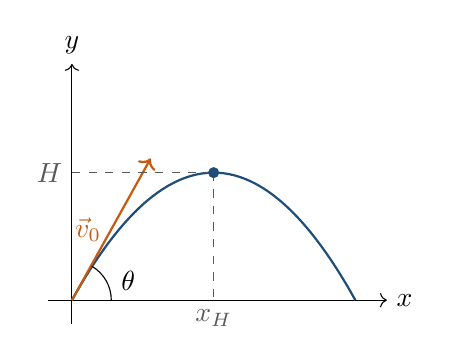
\begin{tikzpicture}
    % 좌표축
    \draw[->] (-0.3,0) -- (4,0) node[right] {$x$};
    \draw[->] (0,-0.3) -- (0,3) node[above] {$y$};
    % 포물선
    \draw[thick, myblue, domain=0:3.6, samples=60]
      plot (\x, {-0.5*\x*\x + 1.8*\x});
    % 초기 속도 벡터
    \draw[->, thick, myorange] (0,0) -- (1.0, 1.8)
      node[midway, left] {$\vec{v}_0$};
    % 각도 표시
    \draw (0.5,0) arc[start angle=0, end angle=60, radius=0.5]
      node[midway, right, xshift=2pt] {$\theta$};
    % 점선 (최고점)
    \draw[dashed, mygray] (1.8, 1.62) -- (1.8, 0) node[below] {$x_H$};
    \draw[dashed, mygray] (0, 1.62) node[left] {$H$} -- (1.8, 1.62);
    \fill[myblue] (1.8, 1.62) circle (2pt);
  \end{tikzpicture}
  \caption{포물선 운동의 궤적}
  \label{fig:projectile}
\end{figure}

%---------------------------------------------------------------
\subsection{pgfplots 그래프 예시}
%---------------------------------------------------------------

\begin{figure}[H]
  \centering
  \begin{tikzpicture}
    \begin{axis}[
      width=0.65\textwidth, height=5cm,
      xlabel={시간 $t\,[\mathrm{s}]$},
      ylabel={변위 $x\,[\mathrm{m}]$},
      xmin=0, xmax=6.5,
      grid=major,
      grid style={dashed, gray!40},
      tick label style={font=\small},
      label style={font=\small},
    ]
      \addplot[thick, myblue, domain=0:6, samples=100]
        {2*sin(deg(x))};
      \addlegendentry{$x(t) = 2\sin t$}
    \end{axis}
  \end{tikzpicture}
  \caption{단순 조화 운동의 변위-시간 그래프}
  \label{fig:shm}
\end{figure}

%---------------------------------------------------------------
\section{표 예시}
%---------------------------------------------------------------

\begin{table}[H]
  \centering
  \caption{물리 상수 일람}
  \label{tab:constants}
  \begin{tabular}{llc}
    \toprule
    상수 & 기호 & 값 \\
    \midrule
    빛의 속도    & $c$ & $3.00 \times 10^8\,\mathrm{m/s}$ \\
    중력가속도   & $g$ & $9.80\,\mathrm{m/s^2}$ \\
    플랑크 상수  & $h$ & $6.626 \times 10^{-34}\,\mathrm{J \cdot s}$ \\
    \bottomrule
  \end{tabular}
\end{table}

%===============================================================
\end{document}
%===============================================================
